\section{Implementation Plan}
The implementation of Data4Help and AutomatedSOS systems is carried on taking into consideration some important factors, such as the complexity of each component and its relations with the other ones. Of course, the implementation plan takes into special consideration the core components which are essential for the whole system and are considered as \say{bottleneck}. 
It is important to fix any flaws as soon as it is detected, so that the correction costs in terms of time are kept the lower possible.
The order in which our system is implemented is the following:

\begin{enumerate}
    \item Model
    \item Central Controller
    \item Account Manager
    \item Third party services, User Services
    \item Emergency Service
    \item Web, Mobile and Wearable Applications
\end{enumerate}
\begin{figure}[H]
    \makebox[\textwidth]{
        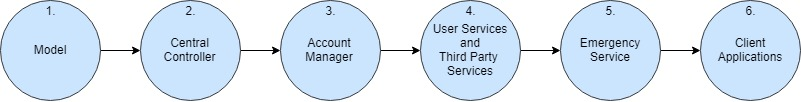
\includegraphics[width=1.3\linewidth]{images/Implementation_plan.jpg}
    }
\end{figure}

\subsubsection{Model}
The Model is the first step of the implementation plan, according to its vital role for the whole application.
Since the classes of the Model are used by all the components, it is important that they are ready as soon as possible and are used as a reference. Otherwise each team member would implement the classes of the Model \say{on the fly} when he/she needs them, introducing possible implementation flaws or not using abstraction in a proper way.

\subsubsection{Central Controller}
This component is the logic core of the application. According to this, it requires lot of time to be implemented and, consequently, it is a risky component. It is important that the least possible flaws are inserted during its implementation, since it may have catastrophic consequences in terms of time costs. An important non functional requirement is the fault tolerance and the high throughput. This component may is stressed with lots of requests by each user and third party and it has to react in a short while. For this reason, this component is consider as a \say{bottleneck}.

\subsubsection{Account Manager}
This module allows the sign-up and login of the users and third parties and also is used by the Central Controller when a third party compose a request for data of a specific user. As shown in the \hyperlink{RV}{\underline{Runtime view, section 2.5}}, the third party fills the request form specifying the user's SSN or Fiscal Code and, thanks to the Account Manager, the Central Controller converts it into the corresponding user ID.
This module is used for the login and sign-up processes by both users and third parties and, consequently, it has to use abstraction to achieve this interdependence.

\subsubsection{Third party services, User Services}
This two components allow the interaction between the user application(mobile or wearable) and the third party application(mobile or web), passing through the Central Controller.
They can be implemented together since they are quit similar to each other.
As shown in the \hyperlink{CV}{\underline{Component view, section 2.5}}, the sub-components that allows the login, the registration and the access to data are the same in the two module. 
Regarding to the Individual and the group requests, the Third party services component offers the possibility to create them while the User services component allow the user to manage them.
According to what just said, they are implemented just after the Central Controller and the Account Manager.

\subsubsection{Emergency Service}
This component has a vital role for the AutomatedSOS system. It analysis real-time health parameters by comparing them with specific thresholds. It has a strictly dependence with the User services component and with the Central Controller, so that it has to be implemented just after they are ready to use.
Of course, Emergency Service has to be fault tolerant since it deals with human lives. In this component, in the case that a fault appears, it has to be recovery as soon as possible since the system must result available 24/7. 
This component must guarantee an high throughput since it receives a large amount of real-time health data from all the users at the same time.

\subsubsection{Web, Mobile and Wearable Applications}
The last part of the system that has to be implemented consists on the applications. They allow user and third party to interacts with the system, so that they don't have a core function for the system.
They represent only a minimum part of the code and they require short while to be implemented. 
Their implementation will be independent from the Operative System of the device on which they will run.
The application must properly run on different devices concerning the users(smart-phones and wearable-devices) and concerning the third parties(personal computers, tablets and smart-phones). 
For these reasons, application components are not considered \say{risky} and they are taking into consideration as the last part of the implementation plan.

\clearpage
\section{Integration and Testing}
\subsection{Entry Criteria}
Integration testing is an important process that has to start as soon as every component is almost complete, so that is possible to promptly fix any flaw that will eventually occur. \\
The purpose of this process is to test the integration between the components of our system, according to all the functionalities listed in the RASD and the DD documents that our application will be able to offer. \\
To start the Integration each component has to correctly pass its unit test.
All the services provided by external entities, including each APIs (Google maps API and the API of the health sensors), have to be completed and they have to properly work since our system will strictly depends on them. For the same reason, also the DBMS and the Data Manager service must be completed before starting all tests. \\
Regarding the AutomatedSOS system-to-be, we have already explained how the interaction between the system and the National Health Services can change according the host country. In the nations in which the NHS provides an API, the latter must be completed before starting the integration tests. Otherwise, there must be an operative VoIP API that allows AutomatedSOS to interact with the NHS.\\ \\
The integration process between two components should start when both of them have reached a minimum level of completion, in order to make the integration tests meaningful.\\
To be detailed, the estimated completion of each component to enter the integration process should be:
\begin{itemize}
    \item Data Manager, \textbf{100\% of completion}
    \item Central Controller, \textbf{90\% of completion}
    \item Account Manager, \textbf{70\% of completion}
    \item Third Party Services, \textbf{60\% of completion}
    \item User Service, \textbf{60\% of completion}
    \item Emergency Services, \textbf{80\% of completion}
    \item Third Party Client Applications, \textbf{40\% of completion}
    \item User Client Applications, \textbf{40\% of completion}
\end{itemize}
In the bulleted list above, the percentages reflect the minimum number of functions that each component must offer in order to enter the integration process.
\clearpage

\subsection{Elements to be Integrated}
As already mentioned in the \hyperlink{SOA_TG}{\underline{Architectural Patterns section}}, the system is based on the Service Oriented pattern which guarantees the modularity and the maintainability of the software. Each component offers some interfaces in order to communicate with the others.
It's important to test the integration of each components to ensure the reliability of the system. \\
Moreover, each requirement listed in the RASD document is achieved thanks to the complex interactions between the interfaces of all the components.\\
We identify four different macro-categories in which components can be grouped, according to their role inside the system.
Referring to the high-level components in the Figure \underline{\ref{HLC}}, we can divide them into:
\begin{itemize}
    \item Client components: third party web application, user mobile application, user wearable application.
    \item Server components: Third party services, user services, account manager, central controller, emergency services.
    \item Data components:  data manager, DBMS.
    \item External components: Maps API, VoIP API, Sensors API.
\end{itemize}
This separation facilitates us in the process of the integration. 
The Server category compose the core logic of the application, so the majority of the interactions takes place inside this category.
On the contrary, there aren't interactions between the components inside the Client categories.\\
In the following lines we list all the elements that need to be integrated together, belonging to the same or different categories.\\ \\
\textbf{Integration of Server Components with Data and External components:}
\begin{itemize}
    \item Central Controller
    \begin{itemize}
        \item Data Provider, Data Manager
        \item Data Gatherer, Data Manager
    \end{itemize}
    \item User Services
    \begin{itemize}
        \item Data Acquisition Manager, Sensors API
        \item Access to Data, Maps API
    \end{itemize}
    \item Third Party Services
    \begin{itemize}
        \item Group Request Service, Maps API
        \item Access to Data, Maps API
    \end{itemize}
    \clearpage
    \item Emergency Service
    \begin{itemize}
        \item Data Analyzer, Data Manager
        \item NHS Adapter, NHS API
    \end{itemize}
\end{itemize}

\textbf{Integration between Server Components:}
\begin{itemize}
    \item Central Controller
    \begin{itemize}
        \item Individual Request Manager, Requests Manager (User Services)
        \item Individual Request Manager, Notification Manager (User Services)
    \end{itemize}
    \item User Services
    \begin{itemize}
        \item Data Sending Service, Data Gathering (Central Controller)
        \item Login Service, Account Manager
        \item Registration Service, Account Manager
    \end{itemize}
    \item Third Party Services
    \begin{itemize}
        \item Individual Request Service, Individual Request Manager (Central Controller)
        \item Group Request Service, Group Request Manager (Central Controller)
        \item Access to Data, Data Provider (Central Controller)
        \item Login Service, Account Manager
        \item Registration Service, Account Manager
    \end{itemize}
    \item Emergency Service
    \begin{itemize}
        \item Data Analyzer, Data Provider (Central Controller)
        \item Emergency Manager, Account Manager (Central Controller)
        \item User Communication Manager, Notification Manager (User Services)
    \end{itemize}
\end{itemize}

\textbf{Integration of Client Components with Server Components:}
\begin{itemize}
    \item User Web, Mobile and Wearable Applications, User Services
    \item Third Party Web and Mobile Applications, Third Party Services
\end{itemize}

\clearpage
\subsection{Integration Testing Strategy}
According to the development approach of our software, we decided to integrate the components using a mixture of two approaches: the \textbf{Bottom Up} and the \textbf{Critical Module First}.

The \textbf{Bottom Up} approach allows us to test the ready components directly in a real world scenario, without creating some specific stubs. It's important that the external services are available for the integration process from the beginning.\\
As soon as a component or a part of it has been implemented, even before it has passed the unit test, it can be integrated with the already existing ones which lies in the lower levels of the hierarchy. Using this method we are able to find out the reaction of the system in the real world usage, so that we can promptly intervene if something go wrong.\\
We also choose this integration approach since it reflects the same approach used during the implementation phase, so that we can optimize the efficiency of the project.
Components that lies in the same hierarchy level can be integrated in an arbitrary order, maybe integrating the ones that will be ready first.

The Server components represent the core logic of the entire system, so it is necessary to start integrating them from the beginning.
For this reason we also decided to use the \textbf{Critical Module First} approach to start integrating the riskiest components first.
Since a fault in these components may have tragic consequences for the entire system, this approach allows us to fix the bugs earlier.

Components provided by external entities, such as \textbf{Maps API}, \textbf{health sensors APIs}, \textbf{NHS API} and \textbf{VoIP API} can be immediately used in the integration since we assume that they are ready before all the others. Also the \textbf{Data Manager} and the \textbf{DBMS} components have to be completed before starting the integration, since the lower level of the hierarchy strongly depends on them.\\
\subsection{Sequence of Component/Function Integration}
This section illustrates the plan of the integration between components of our systems. The following diagrams represents a model of the integration order. An arrow going from component X to component Y means that Y is necessary for X functioning, so it must have already been implemented before integration happens.

\subsubsection{Software Integration Sequence}
\begin{figure}
    \centering
    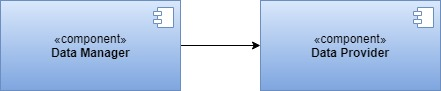
\includegraphics[width=295pt]{images/IntegrationSequence/TrackMe-Integration_sequence1.jpg}
    \caption{The third party obtains the requested data.}
\end{figure}
\begin{figure}
    \centering
    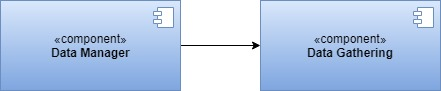
\includegraphics[width=295pt]{images/IntegrationSequence/TrackMe-Integration_sequence2.jpg}
    \caption{The third party obtains the requested data.}
\end{figure}
\begin{figure}
    \centering
    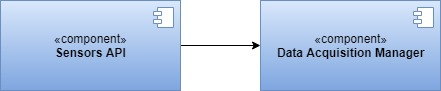
\includegraphics[width=295pt]{images/IntegrationSequence/TrackMe-Integration_sequence3.jpg}
    \caption{The third party obtains the requested data.}
\end{figure}
\begin{figure}
    \centering
    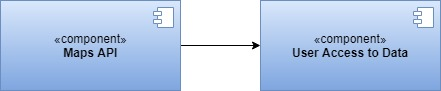
\includegraphics[width=295pt]{images/IntegrationSequence/TrackMe-Integration_sequence4.jpg}
    \caption{The third party obtains the requested data.}
\end{figure}
\begin{figure}
    \centering
    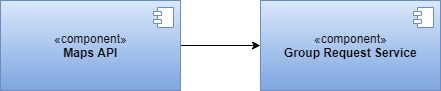
\includegraphics[width=295pt]{images/IntegrationSequence/TrackMe-Integration_sequence5.jpg}
    \caption{The third party obtains the requested data.}
\end{figure}
\begin{figure}
    \centering
    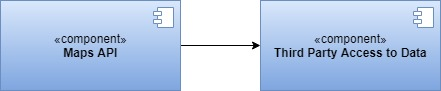
\includegraphics[width=295pt]{images/IntegrationSequence/TrackMe-Integration_sequence6.jpg}
    \caption{The third party obtains the requested data.}
\end{figure}
\begin{figure}
    \centering
    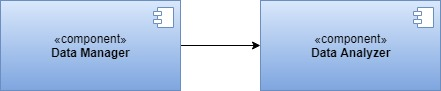
\includegraphics[width=295pt]{images/IntegrationSequence/TrackMe-Integration_sequence7.jpg}
    \caption{The third party obtains the requested data.}
\end{figure}
\begin{figure}
    \centering
    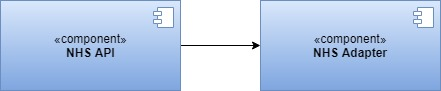
\includegraphics[width=295pt]{images/IntegrationSequence/TrackMe-Integration_sequence8.jpg}
    \caption{The third party obtains the requested data.}
\end{figure}
\begin{figure}
    \centering
    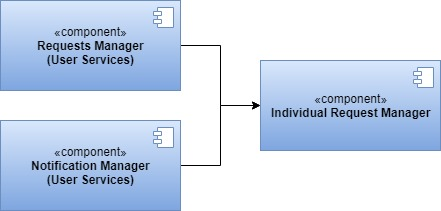
\includegraphics[width=295pt]{images/IntegrationSequence/TrackMe-Integration_sequence9.jpg}
    \caption{The third party obtains the requested data.}
\end{figure}
\begin{figure}
    \centering
    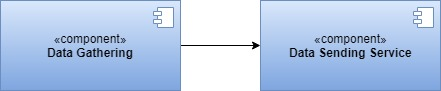
\includegraphics[width=295pt]{images/IntegrationSequence/TrackMe-Integration_sequence10.jpg}
    \caption{The third party obtains the requested data.}
\end{figure}
\begin{figure}
    \centering
    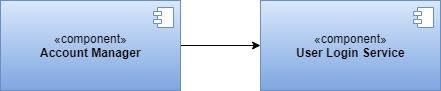
\includegraphics[width=295pt]{images/IntegrationSequence/TrackMe-Integration_sequence11.jpg}
    \caption{The third party obtains the requested data.}
\end{figure}
\begin{figure}
    \centering
    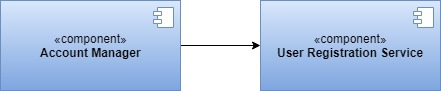
\includegraphics[width=295pt]{images/IntegrationSequence/TrackMe-Integration_sequence12.jpg}
    \caption{The third party obtains the requested data.}
\end{figure}
\begin{figure}
    \centering
    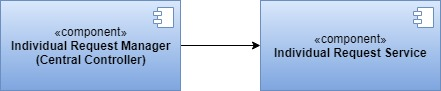
\includegraphics[width=295pt]{images/IntegrationSequence/TrackMe-Integration_sequence13.jpg}
    \caption{The third party obtains the requested data.}
\end{figure}
\begin{figure}
    \centering
    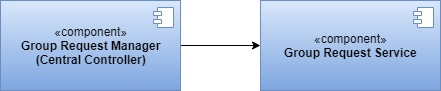
\includegraphics[width=295pt]{images/IntegrationSequence/TrackMe-Integration_sequence14.jpg}
    \caption{The third party obtains the requested data.}
\end{figure}
\begin{figure}
    \centering
    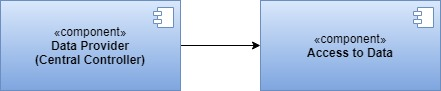
\includegraphics[width=295pt]{images/IntegrationSequence/TrackMe-Integration_sequence15.jpg}
    \caption{The third party obtains the requested data.}
\end{figure}
\begin{figure}
    \centering
    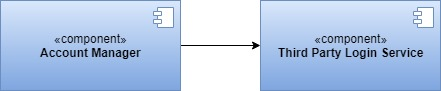
\includegraphics[width=295pt]{images/IntegrationSequence/TrackMe-Integration_sequence16.jpg}
    \caption{The third party obtains the requested data.}
\end{figure}
\begin{figure}
    \centering
    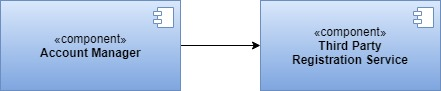
\includegraphics[width=295pt]{images/IntegrationSequence/TrackMe-Integration_sequence17.jpg}
    \caption{The third party obtains the requested data.}
\end{figure}
\begin{figure}
    \centering
    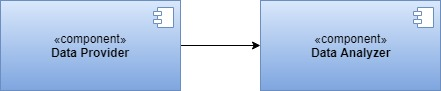
\includegraphics[width=295pt]{images/IntegrationSequence/TrackMe-Integration_sequence18.jpg}
    \caption{The third party obtains the requested data.}
\end{figure}
\begin{figure}
    \centering
    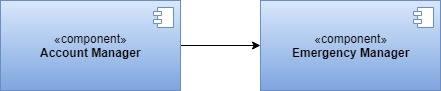
\includegraphics[width=295pt]{images/IntegrationSequence/TrackMe-Integration_sequence19.jpg}
    \caption{The third party obtains the requested data.}
\end{figure}
\begin{figure}
    \centering
    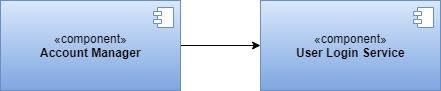
\includegraphics[width=295pt]{images/IntegrationSequence/TrackMe-Integration_sequence20.jpg}
    \caption{The third party obtains the requested data.}
\end{figure}
\begin{figure}
    \centering
    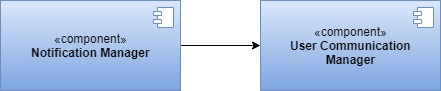
\includegraphics[width=295pt]{images/IntegrationSequence/TrackMe-Integration_sequence21.jpg}
    \caption{The third party obtains the requested data.}
\end{figure}
\clearpage
\subsubsection{Subsystem Integration Sequence}
\begin{figure}[H]
    \makebox[\textwidth]{
        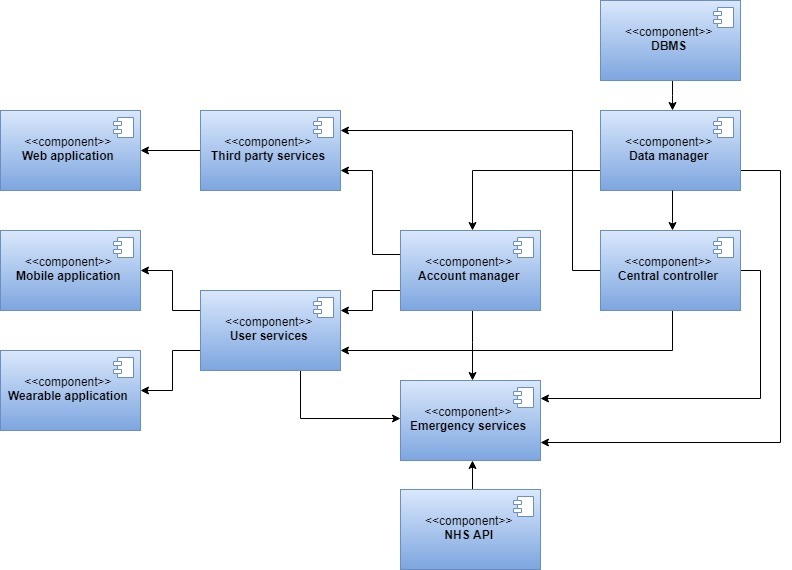
\includegraphics[width=1.4\linewidth]{images/IntegrationSequence/Subsystem_Integration_sequence.jpg}
    }
\end{figure}